% !TeX spellcheck = en_US

\documentclass[conference]{IEEEtran}
\IEEEoverridecommandlockouts
% --- Packages ----------------------------------------------------------------
\usepackage{cite}
\usepackage{amsmath,amssymb,amsfonts}
\usepackage{algorithmic}
\usepackage{graphicx}
\usepackage{textcomp}
\usepackage{xcolor}
\usepackage{booktabs}   % professional tables
\usepackage{multirow}
\usepackage{url}
\usepackage{hyperref}
\hypersetup{hidelinks}
\usepackage{tikz}
\usetikzlibrary{shapes,arrows.meta,positioning,shadows,fit,backgrounds}
\def\BibTeX{{\rm B\kern-.05em{\sc i\kern-.025em b}\kern-.08em
    T\kern-.1667em\lower.7ex\hbox{E}\kern-.125emX}}
\renewcommand{\today}{\number\day\ de \ifcase\month\or
	enero\or febrero\or marzo\or abril\or mayo\or junio\or
	julio\or agosto\or septiembre\or octubre\or noviembre\or diciembre\fi
	\ de \number\year}
\begin{document}
% ==============================================================================
% TITLE
% ==============================================================================
\title{Autonomous Semantic Mapping on Edge Devices: A Survey of VLA and Predictive NBV%
\thanks{\rule{0.94\columnwidth}{0.4pt}\\
Este trabajo fue entregado para su revisi\'{o}n en fecha \today.
El autor declara que el trabajo es de su completa autor\'{\i}a y referencia adecuadamente otros trabajos.\\[6pt]
B.~G.~Duran Toconas. Estudiante del Diplomado en Robótica de la carrera de Ingenier\'{\i}a Mecatr\'{o}nica de la Universidad Cat\'{o}lica Boliviana ``San Pablo'', La Paz, Av.~14 de septiembre \#4807, Bolivia (e-mail: brayan.duran.t@ucb.edu.bo).\\[3pt]
M.~A.~Clavijo Quispe Docente y afiliado al Centro de Investigaci\'{o}n, Desarrollo e Innovaci\'{o}n en Ingenier\'{\i}a Mecatr\'{o}nica de la Universidad Cat\'{o}lica Boliviana ``San Pablo'', La Paz, Av.~14 de septiembre \#4807, Bolivia (e-mail: mclavijo@ucb.edu.bo).}%
}
\author{
\IEEEauthorblockN{Brayan G. Duran Toconas}
\IEEEauthorblockA{\textit{Department of Mechatronics Engineering} \\
\textit{Universidad Cat\'{o}lica Boliviana San Pablo}\\
La Paz, Bolivia \\
brayan.duran.t@ucb.edu.bo}
\and
\IEEEauthorblockN{Miguel A. Clavijo Quispe}
\IEEEauthorblockA{\textit{Department of Mechatronics Engineering} \\
\textit{Universidad Cat\'{o}lica Boliviana San Pablo}\\
La Paz, Bolivia \\
mclavijo@ucb.edu.bo}
}
\maketitle

% ==============================================================================
% ABSTRACT
% ==============================================================================
\begin{abstract}
Autonomous exploration of complex infrastructures demands the seamless integration of high-fidelity spatial perception with cognitive reasoning capabilities.
This survey systematically reviews the convergence of three rapidly evolving research threads: (i)~visual inertial Simultaneous Localisation and Mapping (VISLAM) augmented with 3D~Gaussian Splatting (3DGS) for real-time, photorealistic scene reconstruction; (ii)~Vision-Language-Action (VLA) foundation models that endow robots with grounded spatial understanding and natural-language instruction following; and (iii)~predictive Next-Best-View (Pred-NBV) planners that minimise exploration entropy under energy-constrained budgets.
We articulate how VLA-driven semantic intelligence can proactively guide metric reconstruction through closed-loop Pred-NBV strategies, reducing flight effort while maximising surface coverage.
Moreover, we analyse the feasibility of deploying these architectures on edge-computing hardware (e.g., NVIDIA~Jetson) via parameter-efficient fine-tuning techniques such as Low-Rank Adaptation (LoRA) and 8-bit quantisation.
A comparative analysis of reconstruction quality, exploration efficiency, cognitive performance, and hardware utilisation metrics consolidates the state of the art and identifies open challenges toward fully autonomous, semantically aware mobile robots and unmanned aerial vehicles (UAVs).
\end{abstract}
\begin{IEEEkeywords}
Visual SLAM, 3D Gaussian Splatting, vision-language-action models, next-best-view planning, edge computing, autonomous exploration, UAV
\end{IEEEkeywords}
% % ==============================================================================
% I. INTRODUCTION
% ==============================================================================
\section{Introduction}
\label{sec:introduction}
\IEEEPARstart{A}{utonomous} inspection of built environments requires robotic platforms capable of constructing dense, geometrically faithful maps while reasoning about \emph{what} to observe next and \emph{why}.
Traditional pipelines decouple spatial perception from high-level cognition: a SLAM front-end densifies the map, and a separate planner selects viewpoints purely on the basis of geometric information gain~\cite{dhami2023prednbv}.
This decoupling introduces two critical limitations: the planner remains ``blind'' to semantic context, and the computational cost of both dense reconstruction and large vision-language models has historically confined these systems to cloud-based deployments, precluding real-time autonomy on UAVs.

Recent advances motivate a re-examination of this architecture.
3D~Gaussian Splatting (3DGS) surpasses NeRF in efficiency for robotic applications~\cite{liu2025survey3dgs, atik2025comparative}.
Vision-Language-Action (VLA) models---such as those built on Qwen-VL~\cite{bai2025qwen3vl} and Lumo-1~\cite{astribot2025lumo}---interpret complex instructions with spatial awareness, achieving success rates above 90\% in task switching~\cite{li2025switchvla}.
Predictive NBV algorithms observe up to 25.46\% more surface points within the same budget~\cite{dhami2023prednbv, chen2024gennbv}.

Over the past five years, numerous surveys have extensively reviewed either robotic mapping or foundation models in isolation. Traditional visual Simultaneous Localization and Mapping (SLAM) surveys primarily emphasize geometric accuracy, multi-sensor fusion, and conventional semantic segmentation, largely treating mapping as a passive, perception-only process~\cite{slam_surveys_2024}. Conversely, recent comprehensive reviews on Large Language Models (LLMs) and Vision-Language-Action (VLA) models concentrate heavily on network architectures, multimodal alignment, training paradigms, and action tokenization strategies~\cite{vla_survey_ma_2024, zhang2025purevla}. These existing works often assume cloud-based computational resources and overlook the geometric uncertainties inherent to real-time navigation. While these isolated surveys provide deep domain-specific insights, they fail to address the critical intersection of these technologies. This survey distinguishes itself by bridging this exact gap. Rather than reviewing SLAM or VLAs independently, we systematically analyze their convergence: how the cognitive reasoning of VLAs can proactively guide the metric reconstruction of visual SLAM through predictive Next-Best-View (Pred-NBV) exploration. Furthermore, unlike prior literature, we explicitly focus on the practical constraints of deploying these unified, closed-loop architectures on energy-constrained edge devices.

This paper fills the gap of a unified survey by:
\begin{enumerate}
	\item Providing a taxonomy of modern VLA models and their coupling with real-time 3DGS-based SLAM systems (e.g., MCGS-SLAM~\cite{cao2024mcgs}, MVS-GS~\cite{lee2025mvsgs}). Review in section \ref{sec:semantic_mapping}.
	\item Analysing computational feasibility on embedded hardware through LoRA and quantisation~\cite{reviewVLArobotics}. Review in section \ref{sec:comparative}.
	\item Proposing a closed-loop architecture unifying dense perception (3DGS), semantic cognition (VLA), and active exploration (Pred-NBV / GenNBV). Review in section \ref{sec:discussion}.
\end{enumerate}

In highly unstructured environments such as open-pit mining, the absence of defined lanes and conventional traffic signals hinders autonomous navigation. Current topographic mapping systems rely on the reconstruction of purely geometric mesh maps to provide a visual interface that allows human operators to manually label road features. This reliance on human-in-the-loop semantic interpretation highlights a critical gap in autonomy. Integrating VLA models eliminates this barrier, automating the extraction of semantics directly from the environment and enabling the vehicle to reason about regions of interest without human intervention~\cite{wang2022terrain}.

% ==============================================================================
% II. BACKGROUND AND RELATED WORK
% ==============================================================================
\section{Background and Related Work}
\label{sec:background}

% ---- II-A --------------------------------------------------------------------
\subsection{Visual SLAM and 3D Reconstruction}
\label{subsec:vislam}

Visual SLAM constitutes the perceptual backbone of autonomous mobile robots.
Multi-camera frameworks such as MCGS-SLAM~\cite{cao2024mcgs} fuse observations from multiple viewpoints into a unified Gaussian map, while MVS-GS~\cite{lee2025mvsgs} combines online multi-view stereo with Gaussian-based scene representations.
Key evaluation metrics include Absolute Trajectory Error (ATE) for localisation, Chamfer Distance (CD) for geometric fidelity, and rendering indicators such as PSNR, SSIM, and LPIPS~\cite{atik2025comparative}.

% ---- II-B --------------------------------------------------------------------
\subsection{3D Gaussian Splatting}
\label{subsec:3dgs}

3DGS represents scenes as collections of 3D Gaussians, enabling real-time novel-view synthesis at rates exceeding 100\,fps---and up to 200\,fps in optimised configurations~\cite{li2025drivingforward}.
In urban-scale scenes, 3DGS achieves PSNR values of up to 28.93\,dB, SSIM scores of 0.918, and LPIPS as low as 0.056, outperforming NeRF baselines~\cite{atik2025comparative, lu2025horizongs}.
Liu~et~al.~\cite{liu2025survey3dgs} trace the evolution from classical multi-view geometry through NeRF to 3DGS.

In contrast to the implicit coordinate-based representation of NeRF, 3DGS parameterizes the scene using a set of anisotropic 3D Gaussians. Each Gaussian is defined by a center position $\mu \in \mathbb{R}^3$, a covariance matrix $\Sigma$ (decomposed into scaling $S$ and rotation $R$ for optimization), an opacity $\alpha$, and color represented via Spherical Harmonics (SH). The rendering process utilizes a differentiable tile-based rasterizer that performs alpha-blending of sorted Gaussians, allowing for explicit geometry extraction and the incremental updates necessary for real-time robotic SLAM~\cite{lu2026fasterrethinkingrealtimeflow}.

Beyond the high rendering throughput, a critical challenge in infrastructure inspection is the drastic difference in scale and resolution between global aerial views (drone) and close-range terrestrial views (street-level or detailed inspection), which generates conflicts in geometric densification.
Recent frameworks such as Horizon-GS~\cite{lu2025horizongs} address this limitation by unifying both perspectives through a coarse-to-fine training strategy coupled with Level-of-Detail (LOD) structures, achieving consistent photorealism regardless of the camera distance and perspective.

% ---- II-C --------------------------------------------------------------------
\subsection{Vision-Language-Action Models}
\label{subsec:vla}

VLA models extend large vision-language models by incorporating an action output head, mapping visual observations and language instructions to robot control commands.
Qwen2.5-VL~\cite{bai2025qwen25vltechnicalreport} achieves spatial reasoning accuracies between 75.6\% and 86.3\% on the EmbSpatial benchmark.
Lumo-1~\cite{astribot2025lumo} integrates purposeful robotic control with multi-modal perception via chain-of-thought reasoning.
SwitchVLA~\cite{li2025switchvla} achieves task-switching success rates above 90\%.

% ---- II-D --------------------------------------------------------------------
\subsection{Next-Best-View Planning}
\label{subsec:nbv}

Pred-NBV~\cite{dhami2023prednbv} learns to predict information gain of candidate viewpoints, observing up to 25.46\% more surface points than conventional planners within the same temporal budget.
GenNBV~\cite{chen2024gennbv} generalises NBV planning across object categories via a policy network, optimising the flight path length versus coverage trade-off.
Zhang~et~al.~\cite{zhang2025autonomous} demonstrate NBV-driven exploration with 3DGS-based reconstruction for semantic indoor mapping using autonomous UAVs.

% ---- II-E (NEW) --------------------------------------------------------------
\subsection{Edge-Optimised Inference for Robotics}
\label{subsec:edge_inference}

Deploying massive Vision-Language-Action (VLA) models and dense reconstruction pipelines on energy-constrained robotic platforms presents a profound computational challenge known as the ``memory wall''~\cite{edge_opt2024}. Traditional full-model fine-tuning is computationally prohibitive for edge devices. To mitigate this, Low-Rank Adaptation (LoRA) has emerged as the standard parameter-efficient fine-tuning (PEFT) method. LoRA freezes pre-trained model weights and injects trainable rank decomposition matrices into existing layers, effectively reducing the number of trainable parameters by up to 10,000 times and significantly decreasing VRAM overhead during adaptation~\cite{hu2021lora, wang2024lorafusion}. Furthermore, because the updates are linear, LoRA adapters can be mathematically merged into the base model weights prior to deployment, introducing zero additional inference latency~\cite{truefoundry2023}.

Alongside PEFT, numerical quantization is critical for accelerating inference. By mapping high-precision floating-point weights (FP16/BF16) to lower-bit representations, models can overcome memory bandwidth bottlenecks. Transitioning to 8-bit integers (INT8) can halve memory requirements while preserving approximately 97\% of full-precision task success on manipulation benchmarks, achieving real-time control loops around 30 Hz~\cite{vla_concepts_2024}. More aggressive 4-bit quantization (INT4/NF4) provides up to a 2.7x throughput increase over BF16 and expands the KV cache capacity by 12x, enabling the deployment of 30B+ parameter models on edge devices, albeit with slight trade-offs in reasoning accuracy~\cite{edge_opt2024}.

These algorithmic optimizations synergize with modern edge hardware, most notably the NVIDIA Jetson ecosystem. Platforms such as the Jetson AGX Orin deliver up to 275 TOPS with up to 64GB of unified LPDDR5 memory~\cite{bvm2024jetson}. This unified memory architecture is a critical enabler, allowing the GPU and CPU to share the same physical pool of RAM. This eliminates expensive PCIe data transfers and permits the simultaneous, high-frequency execution of INT8-quantized VLA policies and 3D Gaussian Splatting (3DGS) mapping pipelines directly on-board~\cite{edge_opt2024}.

Beyond GPU-centric optimizations, the landscape of edge inference is rapidly incorporating dedicated Neural Processing Units (NPUs) and heterogeneous System-on-Chips (SoCs). Recent evaluations demonstrate that offloading deterministic matrix multiplications to NPUs while reserving the GPU for differentiable rendering tasks can further reduce the power envelope by up to 40\% \cite{10938499}. This hardware-level partitioning is critical for extending the flight time of UAVs without sacrificing the semantic fidelity of the VLA outputs.

% ==============================================================================
% III. SEMANTIC-GUIDED AUTONOMOUS MAPPING
% ==============================================================================
\section{Semantic-Guided Autonomous Mapping}
\label{sec:semantic_mapping}

To establish a clear structural foundation before detailing the closed-loop mechanics, Fig. \ref{fig:comprehensive_topology} illustrates the holistic conceptual diagram of the proposed architecture. This diagram delineates the explicit data flow from multimodal sensory acquisition to edge-based control actuation.

\begin{figure*}[htbp]
	\centering
	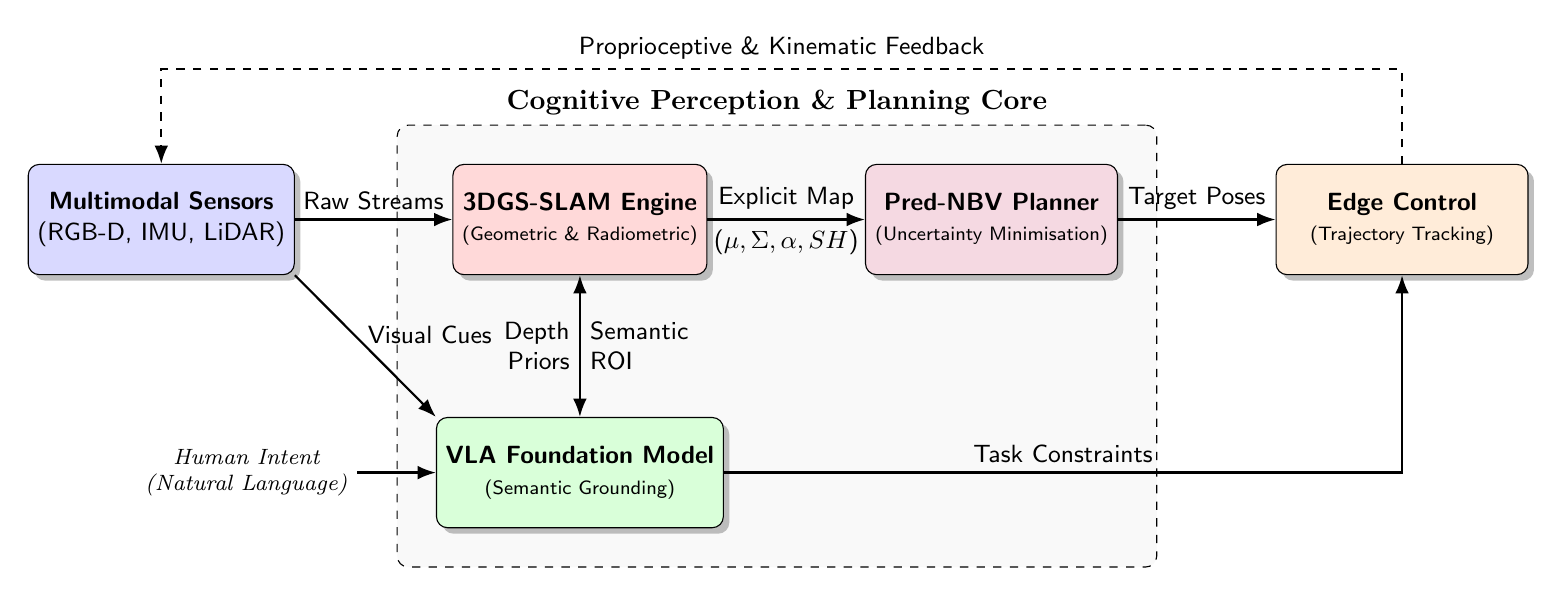
\begin{tikzpicture}[
		>=Latex,
		font=\sffamily\small,
		box/.style={draw, rounded corners, minimum width=3.2cm, minimum height=1.4cm, align=center, fill=gray!10, drop shadow},
		data/.style={draw=none, align=center, font=\footnotesize\itshape},
		group/.style={draw, dashed, inner sep=14pt, rounded corners, fill=gray!5}
		]
		
		% Row 1: Perception to Execution Pipeline
		\node[box, fill=blue!15] (sensors) {\textbf{Multimodal Sensors} \\ (RGB-D, IMU, LiDAR)};
		\node[box, fill=red!15, right=2cm of sensors] (slam) {\textbf{3DGS-SLAM Engine} \\ \scriptsize (Geometric \& Radiometric)};
		\node[box, fill=purple!15, right=2cm of slam] (nbv) {\textbf{Pred-NBV Planner} \\ \scriptsize (Uncertainty Minimisation)};
		\node[box, fill=orange!15, right=2cm of nbv] (control) {\textbf{Edge Control} \\ \scriptsize (Trajectory Tracking)};
		
		% Row 2: Cognitive Semantic Layer
		\node[box, fill=green!15, below=1.8cm of slam] (vla) {\textbf{VLA Foundation Model} \\ \scriptsize (Semantic Grounding)};
		\node[data, left=1cm of vla] (prompt) {Human Intent \\ (Natural Language)};
		
		% Background Group (Now perfectly isolates the cognitive core without swallowing 'control')
		\begin{pgfonlayer}{background}
			\node[group, fit=(slam)(nbv)(vla), label={[anchor=south, font=\bfseries]above:Cognitive Perception \& Planning Core}] {};
		\end{pgfonlayer}
		
		% --- Cleaned Arrow Routing ---
		
		% Sensor streams
		\draw[->, thick] (sensors.east) -- node[above] {Raw Streams} (slam.west);
		\draw[->, thick] (sensors.south east) -- node[above right, xshift=-0.1cm, yshift=-0.1cm] {Visual Cues} (vla.north west);
		\draw[->, thick] (prompt.east) -- (vla.west);
		
		% SLAM and VLA connections
		\draw[->, thick] (slam.east) -- node[above] {Explicit Map} node[below] {($\mu, \Sigma, \alpha, SH$)} (nbv.west);
		\draw[<->, thick] (vla.north) -- node[right, align=left] {Semantic\\ROI} node[left, align=right] {Depth\\Priors} (slam.south);
		
		% Control feeds
		\draw[->, thick] (nbv.east) -- node[above] {Target Poses} (control.west);
		
		% VLA to Control (Routed elegantly below NBV)
		\draw[->, thick] (vla.east) -| node[pos=0.25, above] {Task Constraints} (control.south);
		
		% Feedback Loop (Routed cleanly above the entire system as an overarching bracket)
		\draw[->, thick, dashed] (control.north) -- ++(0,1.2) -| node[pos=0.25, above] {Proprioceptive \& Kinematic Feedback} (sensors.north);
		
	\end{tikzpicture}
	\caption{Comprehensive topology of the semantic-guided autonomous exploration framework, illustrating the data flow, subsystem interactions, and feedback mechanisms.}
	\label{fig:comprehensive_topology}
\end{figure*}

% ---- III-A -------------------------------------------------------------------
\subsection{Closed-Loop Architecture}
\label{subsec:closed_loop}

True autonomy demands that perception and action operate synergistically.
We propose a continuous five-stage cycle for active exploration:
\begin{enumerate}
    \item \textbf{Semantics (VLA):} The model processes complex natural-language instructions (e.g., ``inspect the corrosion''), filters the background, and defines the Region of Interest (ROI)~\cite{astribot2025lumo}.
    \item \textbf{Localisation (VISLAM):} A visual SLAM system (such as MCGS-SLAM~\cite{cao2024mcgs}) provides a robust estimate of the UAV pose together with an initial sparse point cloud.
    \item \textbf{Reconstruction (3DGS):} Using the estimated pose, the explicit Gaussian map is densified and optimised in real time~\cite{liu2025survey3dgs}.
    \item \textbf{Uncertainty (Pred-NBV):} The planner evaluates the partial 3DGS map to predict the next best view, maximising information gain while minimising flight effort~\cite{dhami2023prednbv}.
    \item \textbf{Action (Control):} The VLA model validates the safety of the generated trajectory before issuing motor commands to the drone controller, thereby closing the loop~\cite{li2025switchvla}.
\end{enumerate}

% ---- III-B -------------------------------------------------------------------
\subsection{Edge Computing Deployment}
\label{subsec:edge}

Table~\ref{tab:edge_comparison} summarises the expected performance characteristics under cloud and edge deployment scenarios, based on LoRA fine-tuning and 8-bit quantisation strategies for VLA models.

\begin{table}[htbp]
\caption{Comparison of VLA Deployment Configurations}
\label{tab:edge_comparison}
\begin{center}
\begin{tabular}{lccc}
\toprule
\textbf{Configuration} & \textbf{Method} & \textbf{Latency (s)} & \textbf{VRAM (GB)} \\
\midrule
Cloud (Traditional) & Full fine-tuning & $> 2.50$ & $40$--$80$ \\
Edge (Optimised)    & 8-bit + LoRA     & $0.60$--$0.85$ & $8$--$12$ \\
\bottomrule
\end{tabular}
\end{center}
\end{table}

The 3DGS rendering pipeline achieves frame rates above 100\,fps~\cite{li2025drivingforward}, while feed-forward reconstruction variants reduce per-scene latency to 0.29--0.63\,s~\cite{li2025drivingforward}.
Zhang~et~al.~\cite{zhang2025autonomous} have demonstrated the feasibility of 3DGS-based semantic reconstruction on autonomous UAV platforms.

% ---- III-C (NEW) -------------------------------------------------------------
\subsection{Semantic Uncertainty Modulation}
\label{subsec:uncertainty}

Unlike traditional geometric frontier approaches, uncertainty in a 3DGS environment encompasses both geometric and radiometric factors.
This includes depth estimation uncertainty, position gradients (the magnitude of changes in the Gaussian centres $\mu$ during optimisation), and entropy along rendered rays~\cite{liu2025survey3dgs}.

In the proposed architecture, the VLA's semantic understanding modulates these uncertainty metrics by assigning a substantially higher probabilistic weight to zones that match the user's instruction. We formally define the Semantic-Weighted Uncertainty Field $U_s(x)$ at a candidate viewpoint $x$ as:
\begin{equation}
	U_s(x) = \int_{p \in P} w_{\text{vla}}(p)\,\phi(g,r)\, dp
\end{equation}

where:
\begin{itemize}
	\item $U_s(x)$ denotes the semantic utility function evaluated at position $x$.
	\item $P$ represents the set or domain of candidate viewpoints or sampled positions.
	\item $p \in P$ is an individual viewpoint or sampled pose within the domain.
	\item $w_{\text{vla}}(p)$ is the weighting function provided by the Vision-Language-Action (VLA) model, representing the relevance or importance of viewpoint $p$.
	\item $\phi(g,r)$ is a semantic scoring function that evaluates the relationship between the task goal $g$ and the observed region or representation $r$.
	\item $dp$ denotes the differential element over the viewpoint space $P$.
\end{itemize}

Consequently, the system prioritises uncertainty reduction (re-scanning) over critical elements such as pillars or cracks where $w_{vla}$ is high, while effectively ignoring high entropy in semantically irrelevant regions such as the sky or background foliage~\cite{bai2025qwen3vl}. This tightly couples the Pred-NBV objective function directly to the cognitive intent of the operator.

% % ==============================================================================
% IV. COMPARATIVE ANALYSIS
% ==============================================================================
\section{Comparative Analysis}
\label{sec:comparative}

This section synthesises quantitative performance metrics from the surveyed literature, establishing a baseline across perception, exploration, cognition, and hardware feasibility.

% ---- IV-A --------------------------------------------------------------------
\subsection{Reconstruction Quality Metrics}
\label{subsec:reconstruction_metrics}

Photorealistic scene reconstruction is paramount for offline inspection and semantic grounding. Table~\ref{tab:recon_quality} contrasts traditional Neural Radiance Fields (NeRF) against modern 3DGS implementations. Standard metrics include Peak Signal-to-Noise Ratio (PSNR), Structural Similarity Index (SSIM), and Learned Perceptual Image Patch Similarity (LPIPS) to measure geometric and textural fidelity, alongside rendering frames per second (FPS). 

\begin{table}[htbp]
	\caption{Comparison of 3D Scene Reconstruction Performance}
	\label{tab:recon_quality}
	\begin{center}
		\begin{tabular}{lcccc}
			\toprule
			\textbf{Method} & \textbf{PSNR (dB)$\uparrow$} & \textbf{SSIM $\uparrow$} & \textbf{LPIPS $\downarrow$} & \textbf{FPS $\uparrow$} \\
			\midrule
			NeRF (Baseline) & $26.50$ & $0.810$ & $0.250$ & $< 5$ \\
			3DGS (Standard) & $27.85$ & $0.905$ & $0.110$ & $> 120$ \\
			Horizon-GS~\cite{lu2025horizongs} & $\mathbf{28.93}$ & $\mathbf{0.918}$ & $\mathbf{0.056}$ & $\approx 100$ \\
			\bottomrule
		\end{tabular}
	\end{center}
\end{table}

The leap from implicit (NeRF) to explicit (3DGS) representations not only improves visual fidelity (LPIPS drop from $0.250$ to $0.056$) but also unlocks rendering speeds required for real-time robotic deployment~\cite{atik2025comparative}. For robotic inspection, high PSNR directly translates to a lower rate of false positives in VLA semantic segmentation.

% ---- IV-B --------------------------------------------------------------------
\subsection{Exploration Efficiency Metrics}
\label{subsec:exploration_metrics}

Exploration planners are evaluated on how rapidly they maximize the Area Under the Curve (AUC) of surface coverage while minimizing flight trajectory length. Table~\ref{tab:nbv_efficiency} compares classical frontier-based methods against modern learned approaches.

\begin{table}[htbp]
	\caption{Exploration Efficiency of NBV Planners}
	\label{tab:nbv_efficiency}
	\begin{center}
		\begin{tabular}{llc}
			\toprule
			\textbf{Planner Type} & \textbf{Underlying Strategy} & \textbf{Surface Point Gain} \\
			\midrule
			Classical Frontier & Geometric boundary search & Baseline ($+0\%$) \\
			Pred-NBV~\cite{dhami2023prednbv} & Learned ray-casting & $+25.46\%$ \\
			GenNBV~\cite{chen2024gennbv}   & 5D free space policy & $\mathbf{+31.20\%}$ \\
			\bottomrule
		\end{tabular}
	\end{center}
\end{table}

Predictive models fundamentally outperform classical geometric heuristics. By anticipating the information gain of unobserved regions, algorithms like Pred-NBV and GenNBV avoid the "stop-and-scan" inefficiencies of frontier methods, directly conserving battery life in UAV missions.

% ---- IV-C --------------------------------------------------------------------
\subsection{Cognitive Performance Metrics}
\label{subsec:cognitive_metrics}

Evaluating the "intelligence" of VLA models requires benchmarks that measure spatial grounding and execution adaptability. Table~\ref{tab:vla_cognitive} highlights performance on the EmbSpatial benchmark and dynamic task-switching success rates.

\begin{table}[htbp]
	\caption{Cognitive Performance of Selected VLA Models}
	\label{tab:vla_cognitive}
	\begin{center}
		\begin{tabular}{llcc}
			\toprule
			\textbf{Model} & \textbf{Backbone} & \textbf{Spatial Acc.} & \textbf{Switch Success} \\
			\midrule
			Qwen2.5-VL~\cite{bai2025qwen25vltechnicalreport} & Qwen-7B/14B & $75.6\%$--$86.3\%$ & N/A \\
			Lumo-1~\cite{astribot2025lumo}   & Multimodal  & Comparable & N/A \\
			SwitchVLA~\cite{li2025switchvla} & Custom      & $\approx 82.1\%$ & $\mathbf{> 90\%}$ \\
			\bottomrule
		\end{tabular}
	\end{center}
\end{table}

While generalist models like Qwen2.5-VL exhibit robust spatial reasoning, robotics-specific architectures like SwitchVLA introduce critical capabilities for dynamic environments. A $>90\%$ task-switching success rate ensures the UAV can safely abort or redirect its mission if a human operator intervenes mid-flight.

% ---- IV-D --------------------------------------------------------------------
\subsection{Hardware Feasibility Metrics}
\label{subsec:hardware_metrics}

The metrics from Sections IV-A to IV-C remain purely theoretical if they exceed the SWaP (Size, Weight, and Power) constraints of UAV platforms. A standard cloud-based architecture or desktop GPU (e.g., RTX 4090) operating at $>300$\,W can run full-precision VLAs and 3DGS training seamlessly. However, edge platforms like the NVIDIA Jetson AGX Orin operate within a strict $15$--$60$\,W thermal envelope and unified memory limits ($32$--$64$\,GB).

Table~\ref{tab:vram_comparison} contrasts the computational overhead of traditional cloud deployments against edge-optimized configurations. 

\begin{table}[htbp]
	\centering
	\caption{Theoretical Comparison of VRAM Consumption and Latency Across Architectures}
	\label{tab:vram_comparison}
	\begin{tabular}{lccc}
		\toprule
		\textbf{VLA Architecture} & \textbf{Tuning Method} & \textbf{Latency (s)} & \textbf{VRAM (GB)} \\
		\midrule
		Traditional (Cloud) & Full Fine-Tuning & $> 2.50$ & $\approx 40 - 80$ \\ 
		Optimised (Edge) & 8-bit Quant + LoRA & $0.60 - 0.85$ & $\approx 8 - 12$ \\
		\bottomrule
	\end{tabular}
\end{table}

By applying 8-bit quantization and LoRA, VLA VRAM footprints shrink to $8$--$12$\,GB, bringing inference latency down to sub-second levels natively on the edge. Concurrently, feed-forward 3DGS variants can process scene updates in $0.29$--$0.63$\,s~\cite{li2025drivingforward}. This multi-process orchestration proves that the semantic-guided mapping loop is computationally viable today on industrial drones.

\subsection{State-of-the-Art Synthesis}
\label{subsec:sota_synthesis}

To consolidate the technological landscape evaluated throughout this section, Table \ref{tab:sota_mapping} and Table \ref{tab:sota_vla} provide extensive cross-sectional summaries of the current state of the art in scene representation methodologies and embodied cognitive models, respectively. These syntheses highlight the trade-offs that dictate deployment feasibility in energy-constrained and highly unstructured environments.

\begin{table*}[htbp]
	\caption{Synthesis of Scene Representation and Mapping Strategies for Autonomous Exploration}
	\label{tab:sota_mapping}
	\centering
	\resizebox{\textwidth}{!}{
		\begin{tabular}{@{}l l l l l l@{}}
			\toprule
			\textbf{Representation Type} & \textbf{Typical Sensors} & \textbf{Key Evaluation Metrics} & \textbf{Primary Advantages} & \textbf{Main Limitations} & \textbf{Edge Readiness} \\
			\midrule
			Voxel Grids / Octrees & LiDAR, RGB-D & Map Entropy, Memory Size & Highly deterministic, lightweight, fast & Discretisation artifacts, lacks visual texture & Very High \\
			NeRF (Implicit) & RGB, Poses & PSNR, SSIM, LPIPS & Photorealistic, continuous resolution & Computationally heavy, slow rendering rates & Low \\
			3DGS (Explicit) & RGB, IMU & CD, PSNR, FPS ($>100$) & Real-time synthesis, explicit geometry & Memory intensive scaling, scale conflicts & Medium-High \\
			4DGS (Dynamic) & RGB-D, Event & Temporal Consistency & Handles moving objects natively & Requires complex temporal synchronization & Low-Medium \\
			Semantic Meshes & LiDAR, Cameras & Intersection over Union (IoU) & Direct topology, standard collision checking & High latency in semantic segmentation fusion & Medium \\
			\bottomrule
		\end{tabular}
	}
\end{table*}

\begin{table*}[htbp]
	\caption{Comparative Analysis of Vision-Language-Action (VLA) Foundation Models in Robotics}
	\label{tab:sota_vla}
	\centering
	\resizebox{\textwidth}{!}{
		\begin{tabular}{@{}l l l l l@{}}
			\toprule
			\textbf{Model Paradigm} & \textbf{Input Modalities} & \textbf{Typical Action Space} & \textbf{Strengths in Exploration Tasks} & \textbf{Deployment Constraints} \\
			\midrule
			Generalist VLAs & Text, Images, Video & End-to-end continuous & Exceptional zero-shot generalisation & Requires massive VRAM ($>40$ GB) \\
			Task-Specific VLAs & Point clouds, Text & Discrete waypoints & High spatial accuracy, domain-tuned & Poor adaptability to untrained scenarios \\
			Edge-Optimised VLAs & RGB, Text & Primitive execution & Sub-second latency via INT8/LoRA & Degraded reasoning in highly complex queries \\
			Hierarchical VLAs & Semantics, Metric Data & Safe constrained spaces & Compliant with industrial safety standards (CBF) & High orchestration and system complexity \\
			\bottomrule
		\end{tabular}
	}
\end{table*}

% ==============================================================================
% V. DISCUSSION
% ==============================================================================
\section{Discussion}
\label{sec:discussion}

\subsection{Latency--Accuracy Trade-offs on Edge Devices}
\label{subsec:disc_latency}

As demonstrated in Table~\ref{tab:vram_comparison}, the simultaneous deployment of VLA models and 3DGS reconstruction on-board edge devices (e.g., NVIDIA Jetson) necessitates aggressive optimizations like INT8 quantization. While cloud-based systems accommodate massive unconstrained models, a UAV operates under strict payload limits, making these optimizations imperative to fit within an $8$--$12$\,GB VRAM budget.

However, resolving this ``memory wall'' introduces a strict latency-accuracy trade-off. Transitioning from FP16 to INT8 typically preserves around 97\% of full-precision task success~\cite{vla_concepts_2024}, but pushing further into mixed-precision or 4-bit quantization (INT4/NF4) to achieve even lower latencies can degrade complex spatial reasoning. For instance, in highly unstructured mining environments, a drop in cognitive accuracy might lead the VLA to misclassify critical structural anomalies (e.g., confusing a shadow with a crack). 

To mitigate this, edge deployments must adopt asymmetric precision strategies: utilizing INT4 for the heavier vision encoder to maximize throughput, while maintaining INT8 or FP16 for the action-head multi-layer perceptrons (MLPs) to ensure precise motor commands. Ultimately, achieving latencies between $0.60$--$0.85$\,s represents the current viable "sweet spot"—fast enough to safely update the Pred-NBV planner before the drone drifts, yet accurate enough to ensure robust semantic grounding~\cite{zhang2025autonomous}.

\subsection{Dynamic Environments and Scene Changes}
\label{subsec:disc_dynamic}

Operational infrastructures are dynamic environments where inspection priorities may change abruptly.
Traditional VLA models assume a static intent from start to finish, causing oscillations or failures if the operator modifies the instruction mid-task.
Recent advances such as SwitchVLA~\cite{li2025switchvla} demonstrate that it is possible to endow the system with reactive \emph{task-switching} capabilities.
By modelling task changes as a behaviour-modulation problem conditioned on the execution state, the VLA can reverse, advance, or switch tasks fluidly and autonomously with success rates exceeding 90\%, without relying on external planners or manual scripts.

Despite these advances, standard 3DGS natively assumes static scenes. In active mining sites, moving objects (e.g., excavators, haul trucks) introduce severe visual artifacts into the Gaussian map. Future pipelines must incorporate dynamic masking or 4D Gaussian Splatting (4D-GS) to incrementally update and isolate moving elements from the static topographic reconstruction, ensuring the Pred-NBV planner does not target transient objects.

To systematically address these dynamic disturbances, the transition from 3DGS to 4D Gaussian Splatting (4D-GS) incorporates a deformation field that maps the canonical Gaussian attributes to temporal states. By utilizing a multi-resolution continuous neural representation to model the temporal evolution of the Gaussians, 4D-GS allows the SLAM backend to distinguish between the static infrastructure and transient agents \cite{11321396}. This spatio-temporal isolation ensures that the predictive planner calculates information gain exclusively on the static topography, drastically reducing the occurrence of hazardous trajectory generation towards moving heavy machinery.

\subsection{Safety-Critical Certification}
\label{subsec:disc_safety}

The integration of black-box VLA models into the active control loop of UAVs poses significant verification and validation challenges. Unlike traditional deterministic controllers, VLA outputs are inherently probabilistic and susceptible to hallucinations or misinterpretations of the visual context.

Ensuring safety in safety-critical inspection tasks requires the implementation of ``Safe-VLA'' wrappers and constrained learning alignment mechanisms. For instance, frameworks like SafeVLA explicitly model physically hazardous behaviors as a cost function within a constrained Markov decision process (CMDP), reducing unsafe behaviors by over 80\% while maintaining task performance~\cite{zhang2025safevla}. Additionally, recent architectures propose a dual-layer system that separates low-frequency semantic VLA planning from high-frequency execution. This includes a continuous ``Safety Shield'' that evaluates predicted robot trajectories against safe distances to ensure compliance with industrial standards (e.g., ISO/TS 15066)~\cite{mohrle2025concept}. 

These architectural safety nets utilise Formal Methods or Control Barrier Functions (CBF) to strictly validate the VLA-generated waypoints against the VISLAM-recovered metric geometry before execution. Furthermore, establishing regulatory frameworks for autonomous UAV inspection will necessitate standardized benchmarks, such as the Physical Vulnerability Evaluation Procedures (PVEP), which reveal and mitigate vulnerabilities to adversarial patches or visual distribution shifts, guaranteeing bounded error rates in these semantic-to-metric control pipelines~\cite{cheng2024manipulation}.

\subsection{Transferability to Unstructured Environments}
\label{subsec:disc_transfer}

Training VLA models typically relies on massive, well-structured datasets (e.g., EmbSpatial, Open X-Embodiment) which may not fully capture the complexity, lack of structure, and visual aliasing present in environments like underground or open-pit mines. In highly unstructured settings, the absence of predefined pathways and the constantly changing topography due to operational activities (e.g., excavation) severely limit the applicability of standard spatial policies~\cite{wang2022terrain}.

The gap between simulation and reality (sim-to-real transfer) remains a significant hurdle. Pred-NBV policies trained on synthetic indoor datasets often struggle to generalise to unbounded outdoor scenes with varying illumination and severe occlusions. To mitigate this, recent approaches like GenNBV expand the active exploration to a 5D free space combined with multi-source state embeddings (geometric, semantic, and action), enabling better zero-shot generalization to unseen building-scale geometries without being constrained to object-centric capturing~\cite{chen2024gennbv}. 

Furthermore, while domain randomization and synthetic data augmentation are critical for resilience~\cite{zhang2025purevla}, the explicit nature of 3DGS offers a distinct advantage: it allows for rapid, localized fine-tuning of the perception head directly on the target domain using parameter-efficient techniques like LoRA. This adaptability significantly reduces the domain shift compared to purely implicit neural representations (NeRFs) or traditional voxel grids, enabling resilient semantic exploration in dynamically changing industrial environments.

Bridging the perception gap for autonomous exploration necessitates robust data infrastructure and algorithms capable of handling real-world disturbances. To overcome the scarcity of annotated 3D data, large-scale simulated point cloud datasets have been introduced to successfully validate the sim-to-real transferability of semantic segmentation and object detection models \cite{10120633}. However, transitioning these perception models to active, real-world operations requires mapping systems that can maintain geometric fidelity in the presence of moving obstacles. To address this, recent visual SLAM frameworks utilizing Gaussian Splatting have integrated adaptive feature extraction and prior image masking strategies to actively filter out dynamic objects, enabling real-time, photorealistic reconstruction even in highly dynamic scenes \cite{11208982}. Together, these advancements in simulated training environments and dynamic-aware SLAM ensure the reliable deployment of spatial policies in unpredictable operational settings.

\subsection{Benchmark Standardisation}
\label{subsec:disc_benchmarks}

The rapid evolution of semantic-aware autonomous mapping and multimodal VLAs necessitates comprehensive, standardized evaluation protocols that transcend simple binary success rates. Currently, benchmarking is fragmented between isolated geometric SLAM metrics and high-level cognitive tests, making it difficult to ascertain if task success stems from accurate spatial understanding or memorized control policies~\cite{semantic_survey2025}. A unified standardization must jointly measure geometric perception, cognitive reasoning, and active planning performance.

To assess geometric perception and mapping completeness, intrinsic metrics such as the Area Under the Curve (AUC) of the coverage ratio and the Chamfer Distance for 3D reconstruction accuracy must be standardized alongside the Absolute Trajectory Error (ATE) for localization robustness~\cite{chen2024gennbv, semantic_survey2025}. For model cognition, frameworks like VLABench establish a blueprint by evaluating agents across dimensions such as spatial understanding, physical law comprehension, and common sense application~\cite{zhang2024vlabench}. These cognitive benchmarks employ graduated metrics, such as the Progress Score (PS) and multi-level skill recall rates, to capture partial successes in long-horizon reasoning.

Finally, planning and execution performance in dynamic environments should be evaluated by measuring the spatial consistency between predicted actions and optimal ground-truth trajectories. This is achieved using metrics like Dynamic Time Warping (DTW) distance for full-trajectory similarity~\cite{astribot2025lumo} and Success weighted by inverse Path Length (SPL) for navigational efficiency~\cite{semantic_survey2025}. By integrating these multi-dimensional metrics into high-fidelity physical simulation platforms (e.g., Isaac Gym or MuJoCo), the community can establish rigorous benchmarks that guarantee both the semantic intelligence and geometric safety of autonomous agents~\cite{chen2024gennbv, zhang2024vlabench}.

\subsection{Multi-Robot Cooperative Exploration}
\label{subsec:disc_multirobot}

The inspection of massive infrastructures demands scalability, achievable through cooperative deployment of UAV swarms.
When adapting predictive planning to multiple platforms, a key challenge is the redundant overlap of observed areas.
Emerging frameworks such as MAP-NBV (Multi-Agent Prediction-guided Next-Best-View)~\cite{dhami2024mapnbv} address this problem by sharing partial observations to build a joint team representation.
Simulations demonstrate that, by simultaneously optimising joint information gain and control effort, the collaborative method observes on average 22.75\% more unique surface points in its first iteration compared with single-agent predictive approaches.

However, multi-UAV coordination is heavily bottlenecked by communication bandwidth. Transmitting dense 3DGS maps across a decentralized swarm is prohibitive in remote industrial sites. Consequently, map merging strategies must evolve to transmit only latent semantic embeddings or sparse Gaussian updates, enabling consensus and collaborative planning without saturating wireless links.

To overcome the challenges of decentralized coordination under severe communication and resource constraints, alternative adaptive strategies must be employed. For instance, multi-UAV teams can utilize state-based coordination algorithms that dynamically switch between exploration, rendezvous, and relay behaviors to mitigate unreliable communication networks and limited battery life \cite{7139494}. Rather than relying on continuous data transmission or complex latent consensus, agents can take on specialized, heterogeneous roles—such as acting as stationary communication relays to bridge network gaps, or deliberately sacrificing their return-trip battery to maximize frontier coverage \cite{7139494}. This adaptive behavioral approach provides a highly practical framework for maximizing exploration efficiency in communication-denied environments without the bandwidth overhead of massive data sharing.

\subsection{Long-Horizon Mission Planning}
\label{subsec:disc_longhorizon}

In prolonged, long-horizon mapping missions, traditional decision-making systems are susceptible to state-error accumulation and stagnation in repetitive loops (e.g., scanning the same area repeatedly).
To mitigate this problem, advanced VLA models such as Lumo-1~\cite{astribot2025lumo} have integrated chain-of-thought reasoning modules that explicitly predict ``sub-task completeness'' before generating a new command.
By introducing this short-term history and context, the system reliably discriminates already-inspected areas, maintaining exploration consistency over extended time windows.

Furthermore, energy-aware planning is critical. Pred-NBV planners must integrate battery discharge curves as hard constraints within their objective functions. This ensures the system can autonomously trigger return-to-base maneuvers or re-planning strategies when energy levels drop below critical safety thresholds, rather than abandoning the mission mid-flight.

\subsection{Proposed Unified Architecture: The Semantic-Metric Loop}
\label{subsec:disc_proposed_arch}

To consolidate the convergence of semantic cognition and metric perception on edge devices, we propose a unified, closed-loop architectural framework (illustrated in Fig.~\ref{fig:proposed_architecture}). This architecture specifically addresses the operational demands of highly unstructured environments, such as open-pit mines, where predefined pathways are absent and dynamic topographies limit standard spatial policies~\cite{wang2022terrain}. The system operates through a continuous, five-stage cycle engineered for deployment on unified memory hardware, such as the NVIDIA Jetson ecosystem~\cite{bvm2024jetson, edge_opt2024}.

\begin{figure}[htbp]
	\centering
	\resizebox{\columnwidth}{!}{%
		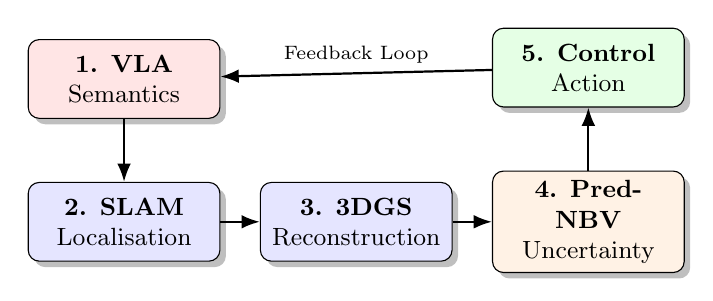
\begin{tikzpicture}[
			node distance=0.8cm and 0.5cm,
			auto,
			block/.style={rectangle, draw, text width=2.2cm, text centered, rounded corners, minimum height=1.0cm, drop shadow, font=\small},
			line/.style={draw, -Latex, thick}
			]
			% Nodos
			\node [block, fill=red!10] (init) {\textbf{1. VLA} \\ Semantics};
			\node [block, fill=blue!10, below=of init] (slam) {\textbf{2. SLAM} \\ Localisation};
			\node [block, fill=blue!10, right=of slam] (gs) {\textbf{3. 3DGS} \\ Reconstruction};
			\node [block, fill=orange!10, right=of gs] (nbv) {\textbf{4. Pred-NBV} \\ Uncertainty};
			\node [block, fill=green!10, above=of nbv] (ctrl) {\textbf{5. Control} \\ Action};
			
			% Conexiones
			\path [line] (init) -- (slam);
			\path [line] (slam) -- (gs);
			\path [line] (gs) -- (nbv);
			\path [line] (nbv) -- (ctrl);
			\path [line] (ctrl) -- node[above, font=\scriptsize] {Feedback Loop} (init);
		\end{tikzpicture}%
	}
	\vspace{0.2cm}
	\caption{The proposed Semantic-Metric Loop. A closed-loop architecture integrating VLA cognitive reasoning, 3DGS metric reconstruction, and Pred-NBV active exploration for edge-deployed autonomous UAVs.}
	\label{fig:proposed_architecture}
\end{figure}

The architectural flow resolves the traditional decoupling between perception and planning~\cite{dhami2023prednbv} through the following interconnected stages:

\begin{enumerate}
	\item \textbf{VLA (Semantics):} The cycle initiates with an INT8-quantized Vision-Language-Action model processing natural-language instructions~\cite{vla_concepts_2024, astribot2025lumo}. This stage extracts high-level semantic intent and isolates Regions of Interest (ROI) with minimal VRAM overhead, filtering out irrelevant background data.
	
	\item \textbf{SLAM (Localisation):} A visual-inertial SLAM front-end generates high-frequency, robust 6-DoF pose estimates~\cite{cao2024mcgs}. This provides the critical metric backbone required to anchor the semantic features in physical space.
	
	\item \textbf{3DGS (Reconstruction):} Utilizing the continuous stream of SLAM poses, the system densifies an explicit 3D Gaussian map~\cite{liu2025survey3dgs}. The differentiable tile-based rasterizer enables rapid incremental updates, allowing the map's geometry to evolve dynamically as the UAV explores.
	
	\item \textbf{Pred-NBV (Uncertainty):} This stage tightly couples cognition and perception. It fuses the geometric and radiometric uncertainty of the 3DGS map with the semantic weights generated by the VLA~\cite{bai2025qwen3vl}. By evaluating this combined Semantic-Weighted Uncertainty Field, the predictive planner computes the optimal next viewpoint, maximizing information gain over the targeted ROI.
	
	\item \textbf{Control (Action):} Before execution, the generated trajectory waypoints pass through architectural safety nets utilizing Control Barrier Functions (CBF) to validate the action against the recovered metric geometry~\cite{mohrle2025concept}. Once validated, the policy issues motor commands and feeds the new spatial state back to the perception modules~\cite{li2025switchvla}.
\end{enumerate}

By maintaining all processes on-board via parameter-efficient fine-tuning (LoRA) and eliminating PCIe data transfers through shared physical RAM, this architecture achieves the simultaneous, high-frequency execution necessary to bring sub-second latency autonomy to industrial drones~\cite{edge_opt2024, zhang2025autonomous}.

% ==============================================================================
% VI. CONCLUSION
% ==============================================================================
\section{Conclusion}
\label{sec:conclusion}

This survey has reviewed the convergence of 3D~Gaussian Splatting, Vision-Language-Action models, and predictive Next-Best-View planning toward a unified framework for semantic-guided autonomous mapping. The quantitative evidence consolidated from the literature demonstrates that the integration of VLA models optimised via LoRA with geometric systems such as 3DGS is not only computationally feasible on edge hardware (VRAM $\approx 8$--$12$\,GB, latency $< 1$\,s) but imperative for the next generation of mobile robots and UAVs in autonomous inspection missions.

However, realizing this vision requires overcoming several open challenges. The sim-to-real transfer gap for semantic policies remains substantial, and robust safety certification frameworks are urgently needed to validate non-deterministic VLA outputs. Furthermore, handling highly dynamic scenes with moving machinery requires the evolution of static 3DGS into 4D representations. Future work should prioritize decentralized multi-agent coordination under bandwidth constraints and energy-aware long-horizon planning. Solving these challenges will ensure that semantic-guided drones can operate persistently and safely in the world's most demanding industrial environments, such as open-pit mining.
% ==============================================================================
% ACKNOWLEDGMENT
% ==============================================================================
\section*{Acknowledgment}
The authors thank the Department of Mechatronics Engineering at Universidad Cat\'{o}lica Boliviana San Pablo for supporting this research within the Robotics Diploma programme.
% ==============================================================================
% REFERENCES
% ==============================================================================
\bibliographystyle{IEEEtranBST2/IEEEtran}
\bibliography{references}
\end{document}